\section{Необходимые условия для полного покрытия с учетом защиты ГСО}
\label{subsec:geo_condition}

% 
Для защиты геостационарных спутников (ГСС) вводится запретная область для 
КА низкоорбитальной группировки. Если угол между направлением из наземной 
точки на КА и направлением на любой видимый из этой точки ГСС меньше предельного 
угла $\varphi$, КА считается создающим помехи и обязан отключить передающий 
луч на данную точку.

Геометрически запретная область представляет собой пересечение сферы 
радиуса $R_{\text{sat}} = R_E + h$ 
(как у нас это обозначается?).
, на которой расположены КА, с 
объединением конусов полураствора $\varphi$. Каждый такой конус строится 
из наземной точки вдоль направления на один из видимых ГСС, а его вершина 
совпадает с этой точкой. Поскольку разные ГСС находятся от неё на разных 
расстояниях, высоты конусов различаются, а углы их пересечения со сферой 
неодинаковы. Это приводит к тому, что запретная область расширяется по мере 
удаления от подспутниковой точки. 

На экваторе эта область симметрична относительно рассматриваемой 
точки и на концах зоны видимости спутника 
(где запретная область имеет самый большой размер) 
имеет угловую полуширину
\begin{equation}
\psi \approx \frac{L \tan\varphi}{R_{\text{sat}}},
\qquad
L = \sqrt{R_E^2 + R_{\text{sat}}^2 - 2 R_E R_{\text{sat}} \cos\theta}.
\label{eq:psi}
\end{equation}

Полуширина вдоль орбиты равна
\begin{equation}
    \alpha =
    \arcsin\!\left(\frac{\sin\psi}{\sin i}\right),
    \label{eq:inplane-alpha}
\end{equation}


С увеличением широты запретная область уменьшается, поскольку увеличивается 
расстояние от точки до ГСО, однако для упрощения мы оцениваем 
её ширину той же величиной $\psi$.

Требование защиты ГСО сводится к тому, что при 
попадании одного КА группировки в запретную область для произвольной 
наземной точки должен найтись другой КА, способный эту точку обслужить. 
Это достигается одним из двух способов: либо уменьшением расстояния 
между КА в одной плоскости либо уменьшением расстояния между соседними плоскостями.

\subsection{Уменьшение расстояния между КА в плоскости}

Для непрерывности покрытия при вынужденном отключении КА, попавшего 
в запретную зону, шаг между соседними КА в плоскости не должен превышать 
угловой размер зоны обзора:
\begin{equation}
\Delta u \le \theta,
\qquad \Delta u = \frac{360^\circ}{S}.
\label{eq:du}
\end{equation}

Рассмотрим прохождение орбиты на рассматриваемой наземной точкой %ToDo сслыка на рисунок и описание
подписей рисунка
Такое размещение позволяет компенсировать отключение КА
в запретной области обслуживанием соседним аппаратом.
При удалении орбиты от рассматриваемой точки доступная для обслуживания
дуга сокращается (ToDo ссылка на тот же рисунок но другой цвет дуги), поэтому дополнительно
требуется ограничить
разность ДВУ соседних плоскостей $\Delta\Omega$.

Предельное положение орбиты определяется моментом,
после которого её собственные КА уже не обеспечивают
непрерывное обслуживание точки. К этому моменту соседняя
орбита должна хотя бы касаться зоны обслуживания
(рис.~\ref{fig:geo-21}). 

\begin{figure}[htbp]
    \centering
    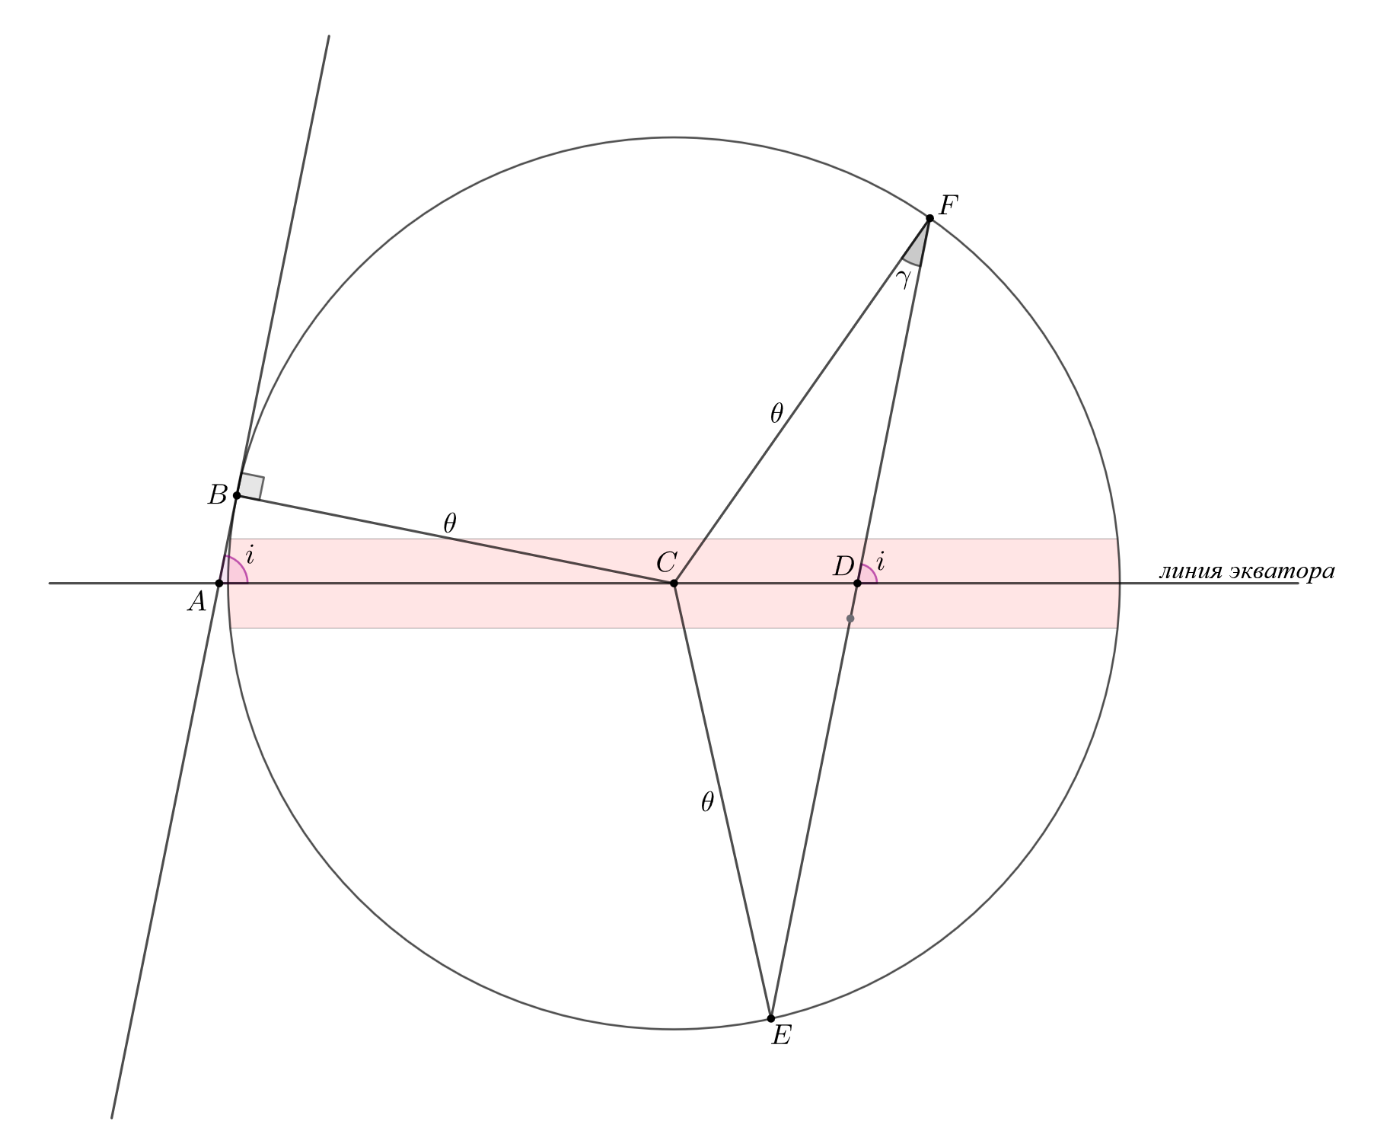
\includegraphics[width=0.55\linewidth]{pictures/geo-fig-21.png}
    \caption{Положение центрального КА относительно запретной
    области. $C$~--- проекция наземной точки на орбитальную сферу;
    $D$~--- восходящий узел; $F$ и $E$~--- границы видимой дуги
    $\widehat{FE}=2\Delta u$; $K$~--- её середина.
    Розовая полоса обозначает запретную область,
    $\alpha$~--- полуширину её пересечения с орбитой,
    $\theta$~--- центральный угол зоны обслуживания,
    $i$~--- наклонение орбиты, $\gamma=\angle CFD$.}
    \label{fig:geo-21}
\end{figure}

%ToDo раскрыть здесь подробнее график fig:geo-21
Геометрия предельного положения зависит от того, находится
ли центральный КА внутри запретной полосы

\paragraph{Центральный КА находится в запретной полосе}
Если $KD\leq\alpha$, то максимальная разность долгот
восходящих узлов составляет
\begin{equation}
    \Delta\Omega_{\max}
    = AC + CD.
    \label{eq:inplane-raan-case1}
\end{equation}

Вспомогательные углы
\begin{align}
    \gamma &=
    \arccos\!\left(\cot\theta\,\tan\Delta u\right),\\
    CD &=
    \arcsin\!\left(
        \frac{\sin\theta\,\sin\gamma}{\sin i}
    \right),\\
    CK &=
    \arccos\!\left(\frac{\cos\theta}{\cos\Delta u}\right),\\
    KD &=
    \arccos\!\left(\frac{\cos CD}{\cos CK}\right).
    AC &= 
    \arcsin\!\left(\frac{\sin\theta}{\sin i}\right)
    \label{eq:inplane-central-position}
\end{align}

\paragraph{Центральный КА находится вне запретной полосы}
Если $KD>\alpha$, то орбиту можно удалить от рассматриваемой точки дальше.
В этом случае предельное положение определяется условием,
что дуга между нижней границей запретной полосы и границей
зоны обслуживания равна $\Delta u$
(рис.~\ref{fig:geo-23}).
Положив $x=\Delta u+\alpha$, получим
\begin{align}
    \beta &=
    \arctan\!\left(\tan x\,\cos i\right),\\
    d_* &=
    \arccos\!\left(
        \frac{\cos\theta}
        {\sqrt{\cos^2x+\sin^2x\cos^2i}}
    \right)+\beta,\\
    \Delta\Omega_{\max}
    &=
    \arcsin\!\left(\frac{\sin\theta}{\sin i}\right)+d_*.
    \label{eq:inplane-raan-case2}
\end{align}

Таким образом, параметры соседних плоскостей должны
удовлетворять условию
\begin{equation}
    \Delta\Omega \leq \Delta\Omega_{\max}.
\end{equation}

Для выбранного $\Delta\Omega$ фазовый сдвиг дополнительно
ограничивается допустимыми участками соседней орбиты:
обслуживающий КА должен находиться внутри зоны обслуживания
и вне запретной полосы в течение отключения КА основной
плоскости. Геометрия допустимых фазовых сдвигов для двух
рассмотренных случаев приведена на
рис.~\ref{fig:geo-24},~\ref{fig:geo-25}.

\begin{figure}[htbp]
    \centering
    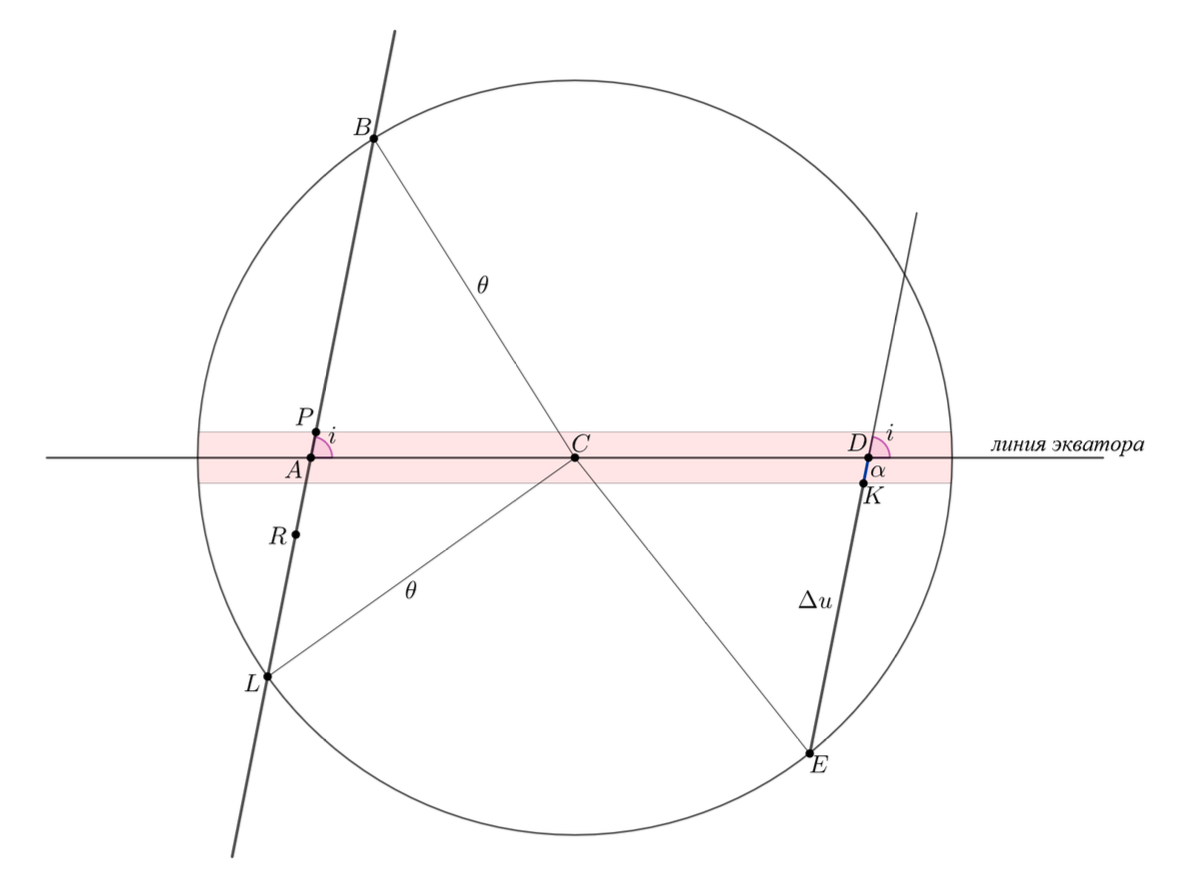
\includegraphics[width=0.55\linewidth]{pictures/geo-fig-24.png}
    \caption{Геометрия фазового
сдвига для случая, когда
средний КА внутри запретной
области}
    \label{fig:geo-24}
\end{figure}

\begin{figure}[htbp]
    \centering
    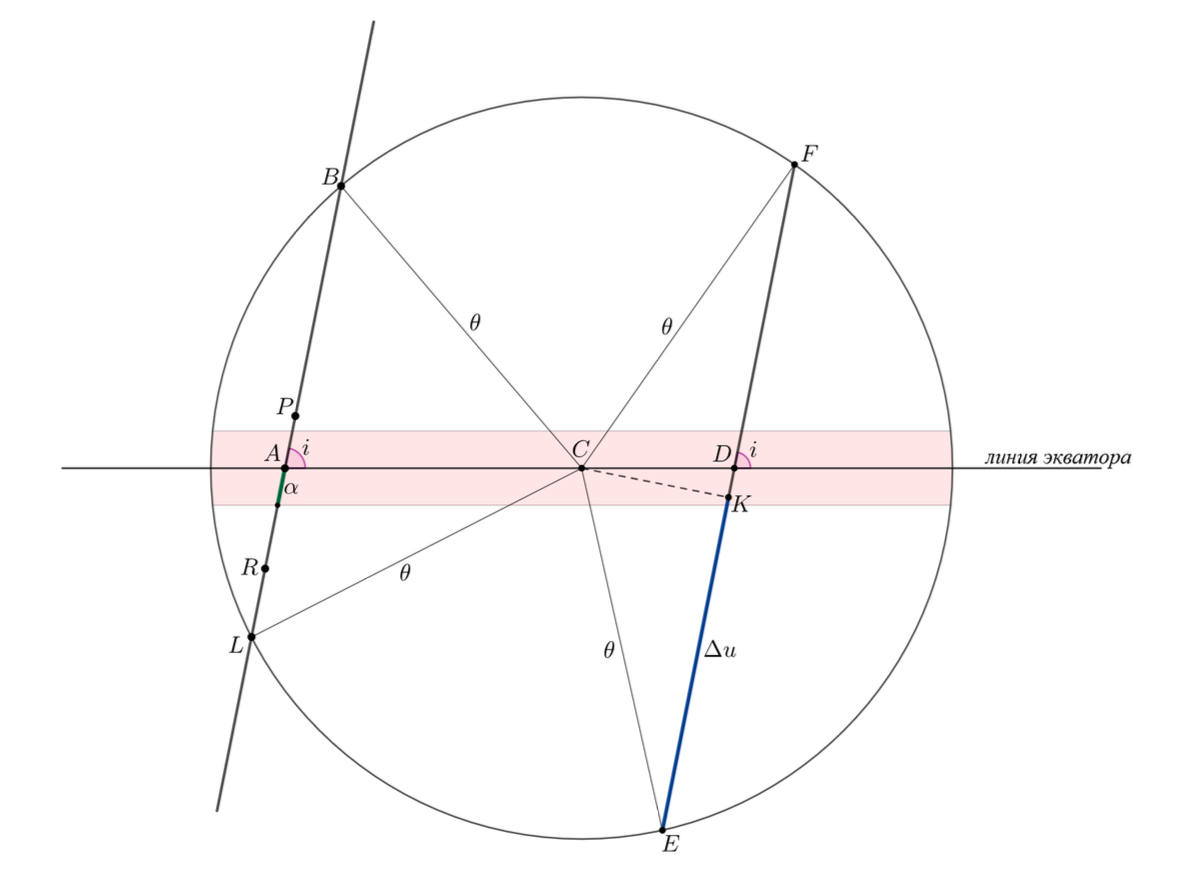
\includegraphics[width=0.55\linewidth]{pictures/geo-fig-25.png}
    \caption{Геометрия фазового
сдвига для случая, когда
средний КА вне запретной
области}
    \label{fig:geo-25}
\end{figure}

Полученные ограничения являются необходимыми условиями
в рамках сферической модели Земли. Их следует применять
совместно с условиями полного геометрического покрытия.



\subsection{Уменьшение расстояния между плоскостями}

Вторая стратегия предполагает уменьшение разности ДВУ
соседних плоскостей $\Delta\Omega$, чтобы при отключении КА
в запретной области наземную точку обслуживали КА соседних
орбит. Рассмотрим точку на экваторе, над которой проходит
основная орбита. Необходимое условие доступности соседней
орбиты определяется её касанием зоны обслуживания
(рис.~\ref{fig:geo-26}):

\begin{equation}
    \Delta\Omega
    \leq
    \arcsin\!\left(\frac{\sin\theta}{\sin i}\right).
    \label{eq:interplane-tangency}
\end{equation}

\begin{figure}[htbp]
    \centering
    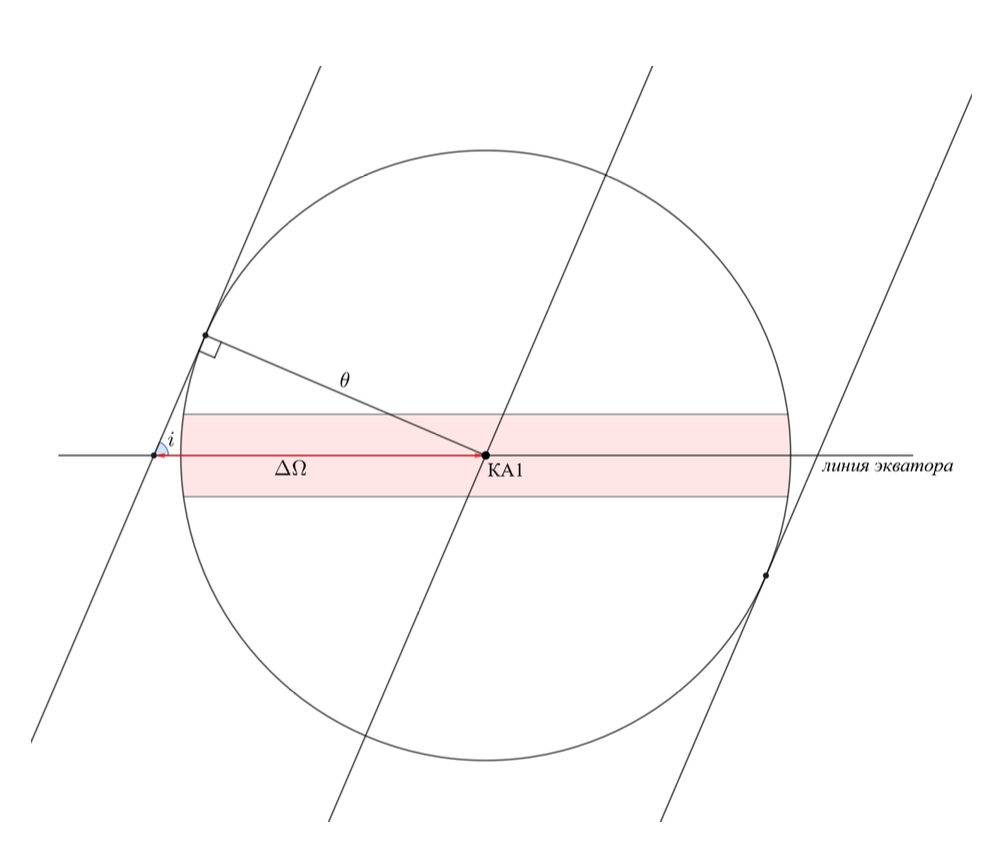
\includegraphics[width=0.55\linewidth]{pictures/geo-fig-26.png}
    \caption{Касание соседней орбитой зоны обслуживания
    экваториальной точки. Основная орбита проходит над точкой;
    соседняя касается границы зоны обслуживания в точке $B$.
    Розовая полоса обозначает запретную область.}
    \label{fig:geo-26}
\end{figure}

Однако касание само по себе не обеспечивает непрерывного
обслуживания. Пока КА основной орбиты проходит запретный
участок, КА соседних орбит должны оставаться внутри зоны
обслуживания и вне запретной полосы.
В рассматриваемой конфигурации это требует, чтобы длина
доступной дуги $\widehat{BB'}$ была не меньше $\alpha$
(рис.~\ref{fig:geo-28}).

\begin{figure}[htbp]
    \centering
    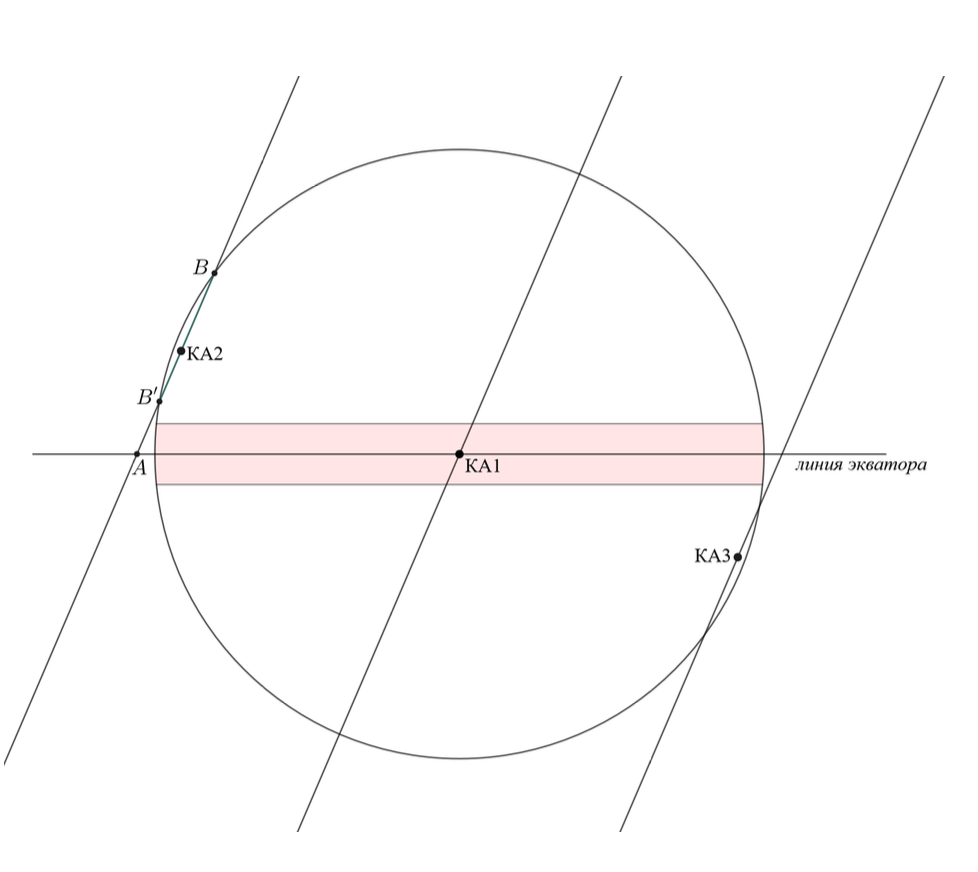
\includegraphics[width=0.47\linewidth]{pictures/geo-fig-27.png}
    \hfill
    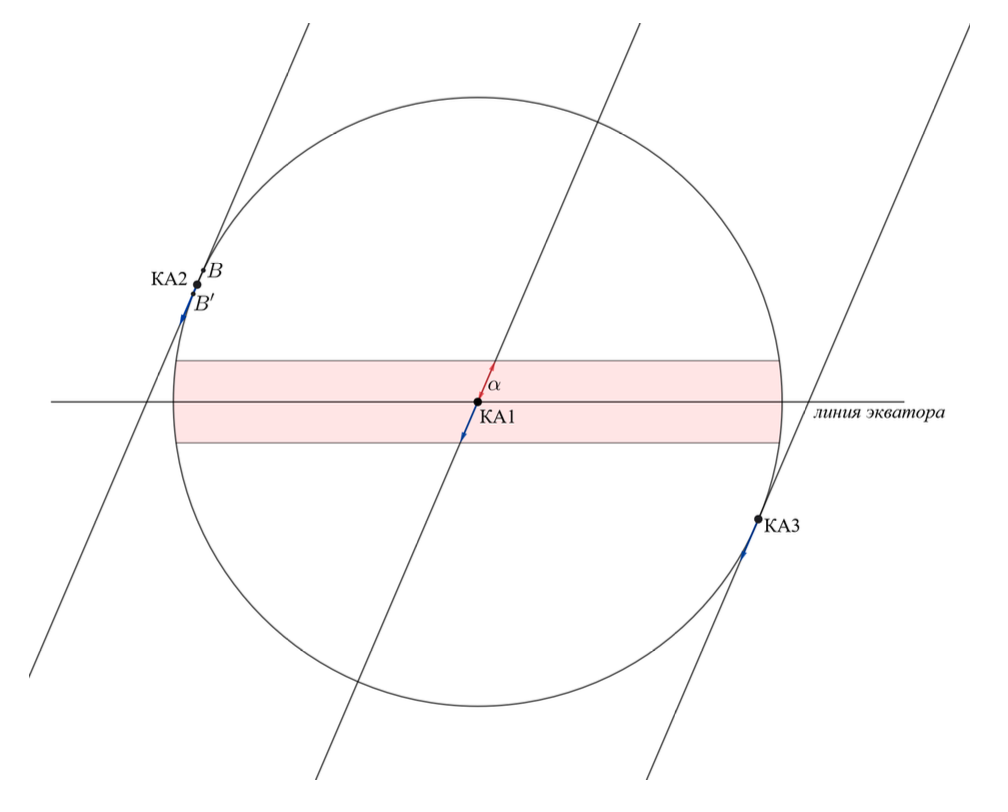
\includegraphics[width=0.47\linewidth]{pictures/geo-fig-28.png}
    \caption{Замещение отключённого КА аппаратами соседних
    орбит. Слева: допустимый участок $\widehat{BB'}$ внутри
    зоны обслуживания и вне запретной полосы.
    Справа: при недостаточной длине этого участка КА2 и КА3
    выходят из зоны обслуживания до выхода КА1 из запретной
    области, что приводит к разрыву покрытия.}
    \label{fig:geo-27}
    \label{fig:geo-28}
\end{figure}

Обозначим через $A$ восходящий узел соседней орбиты,
а через $B$ и $B'$~--- точки её пересечения с границей
зоны обслуживания. Тогда
\begin{equation}
    \widehat{BB'}
    =
    \widehat{AB}-\widehat{AB'}
    =
    2\arccos\!\left(
        \frac{\cos\theta}
        {\sqrt{
            \cos^2\Delta\Omega
            +\sin^2\Delta\Omega\cos^2 i
        }}
    \right).
    \label{eq:interplane-arc}
\end{equation}
Из граничного условия $\widehat{BB'}=\alpha$ получаем
\begin{equation}
    \Delta\Omega_{\max}
    =
    \arcsin\!\left(
        \frac{
            \sqrt{\cos^2(\alpha/2)-\cos^2\theta}
        }{
            \cos(\alpha/2)\sin i
        }
    \right),
    \qquad
    \Delta\Omega\leq\Delta\Omega_{\max}.
    \label{eq:interplane-raan}
\end{equation}
Выражение применяется при допустимых значениях аргумента
арксинуса. Нижняя граница $\Delta\Omega$ определяется
условиями геометрического покрытия между крайними
плоскостями группировки.

\paragraph{Фазовый сдвиг}

Для выбранного $\Delta\Omega$ допустимые положения КА
соседней орбиты определяются видимой дугой за исключением
запретного участка (рис.~\ref{fig:geo-29}).
Введём
\begin{align}
    \eta &=
    \arccos\!\left(
        \frac{\cos\theta}
        {\sqrt{
            \cos^2\Delta\Omega
            +\sin^2\Delta\Omega\cos^2 i
        }}
    \right),\\
    \beta &=
    \arctan\!\left(\tan\Delta\Omega\cos i\right).
\end{align}
Угловые расстояния от восходящего узла $A$ до границ
видимой дуги равны
\begin{equation}
    \widehat{AB}=\eta+\beta,
    \qquad
    \widehat{AL}=\eta-\beta.
    \label{eq:interplane-phase-arcs}
\end{equation}

При соглашении $f=u_{\mathrm{main}}-u_{\mathrm{adj}}$
допустимые фазовые сдвиги составляют
\begin{equation}
    f\in
    [-\widehat{AB},-\alpha]
    \,\cup\,
    [\alpha,\widehat{AL}].
    \label{eq:interplane-phase}
\end{equation}
Первый интервал используется при
$\widehat{AB}\geq2\alpha$, второй~--- при
$\widehat{AL}\geq2\alpha$.
Первое условие обеспечивается выбранной границей
$\Delta\Omega_{\max}$ в рассматриваемой конфигурации.
Если второе условие не выполняется, остаётся только
интервал $[-\widehat{AB},-\alpha]$.

\begin{figure}[htbp]
    \centering
    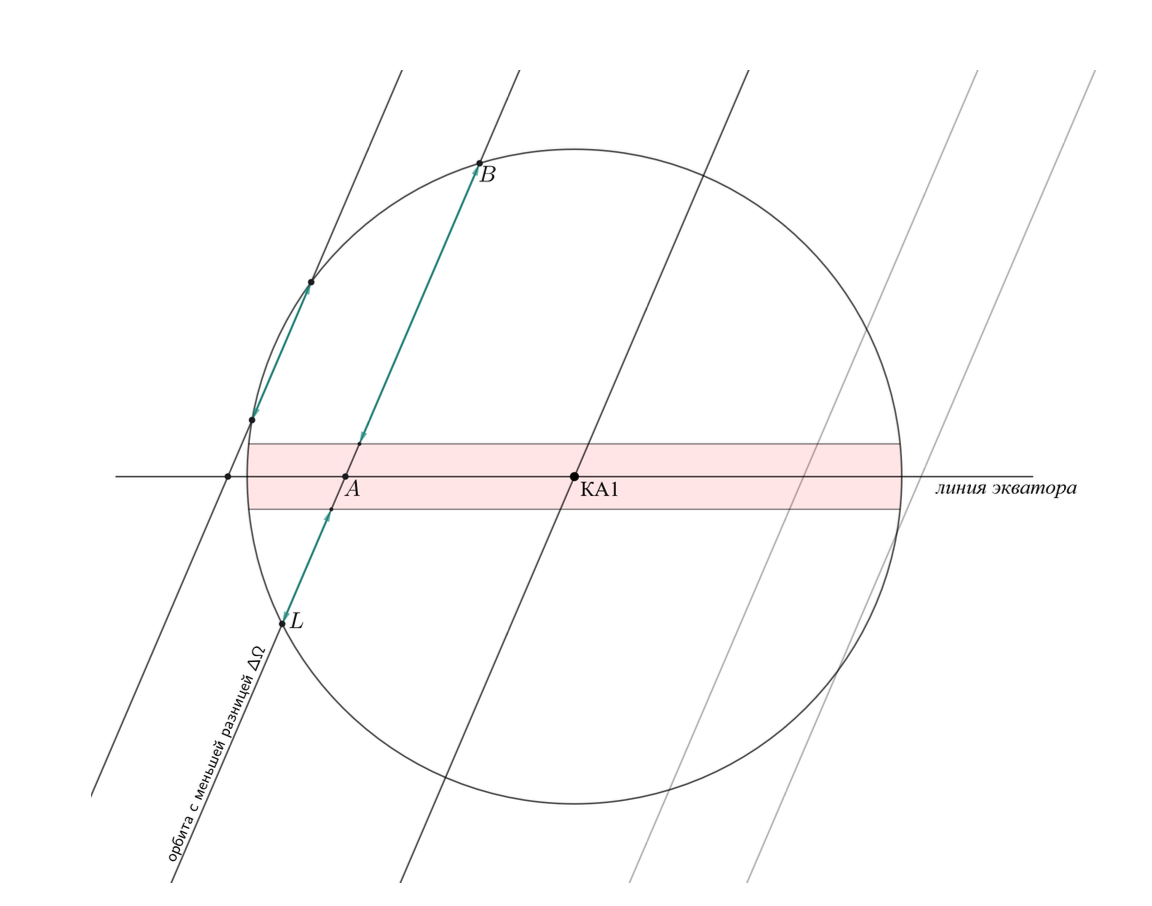
\includegraphics[width=0.55\linewidth]{pictures/geo-fig-29.png}
    \caption{Допустимые положения КА соседней орбиты.
    Точки $B$ и $L$ ограничивают видимую дугу,
    $A$~--- восходящий узел. Зелёным выделены участки
    внутри зоны обслуживания и вне запретной полосы,
    определяющие допустимые фазовые сдвиги.}
    \label{fig:geo-29}
\end{figure}

Ограничение $\widehat{AL}\geq2\alpha$ означает, что
доступная дуга под экватором имеет длину
$\widehat{AL}-\alpha\geq\alpha$.
При меньшей длине обслуживающий КА может покинуть зону
обслуживания раньше, чем КА основной орбиты выйдет
из запретной области (рис.~\ref{fig:geo-30}).

\begin{figure}[htbp]
    \centering
    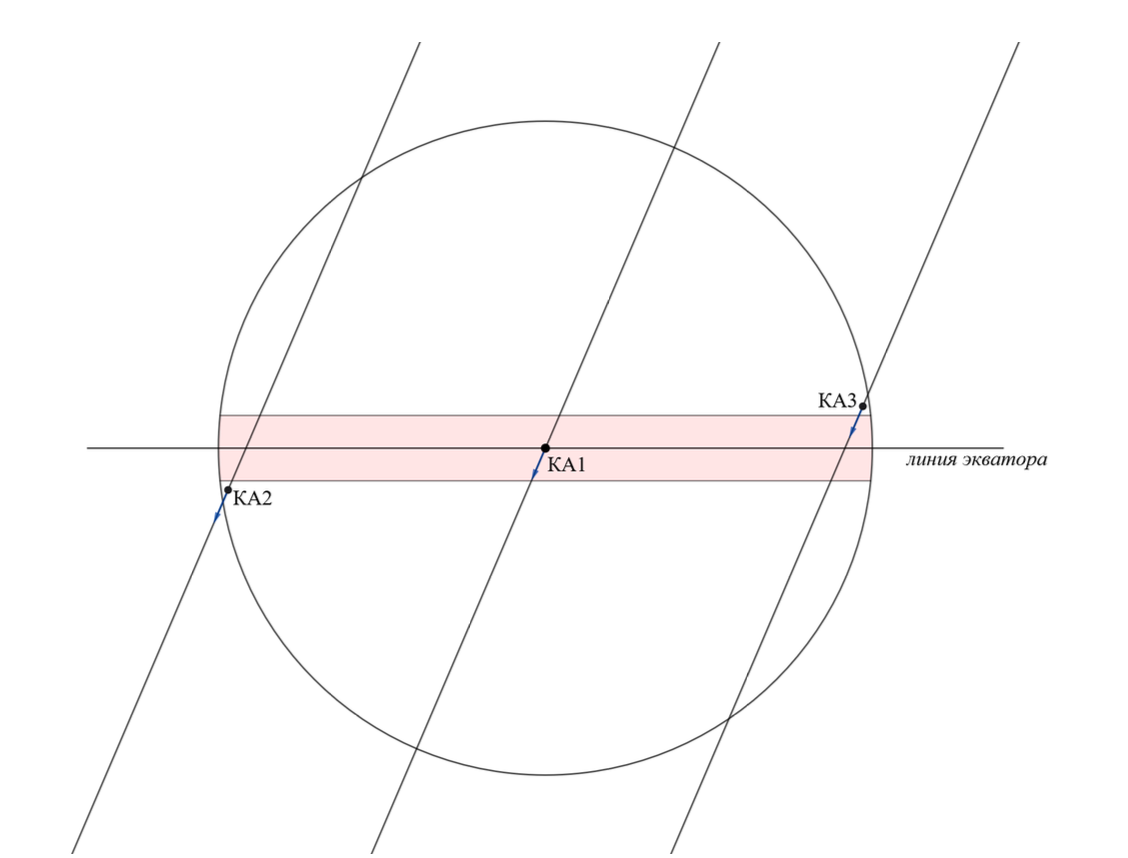
\includegraphics[width=0.55\linewidth]{pictures/geo-fig-30.png}
    \caption{Разрыв покрытия при недостаточной длине
    допустимого участка соседней орбиты под экватором:
    обслуживающие КА выходят из зоны обслуживания,
    пока КА основной орбиты остаётся в запретной области.}
    \label{fig:geo-30}
\end{figure}

Условия \eqref{eq:interplane-raan} и~\eqref{eq:interplane-phase}
являются необходимыми в рассматриваемой модели
и применяются совместно с условиями полного
геометрического покрытия.
